%\addcontentsline{toc}{chapter}{Development Process}
\chapter{Design}

A design specification was produced in the third week of the project. The architecture it proposed will be summarised below and then discussed in the rest of this chapter. The purpose of the design was to consider the project as an entire working system before beginning development. One advantage of creating a design was gaining a better understanding of how the parts of the project needed to fit together. A second incentive was to pre-plan sections of the application considered to be more complicated. These needed more planning, whereas trivial or repetitive aspects of the project were only briefly covered in the design.

The sections of the specification reviewed here are the server API, the database design, the user interface design, and a design for creating a board with positions. The design specification document itself is included in Appendix C.

\section{Overview of the Architecture}
This overview will examine the pieces that make up the main components of the application's architecture.

Research and analysis reached the conclusion that the system would be comprised of two main components: the client side and server side frameworks. AngularJS was the framework of choice for the client side. The server side would be built using Ruby on Rails.

Communication between these two layers would depend on an API following the REST protocol. This means that the server should be designed to represent its resources in compliance with REST, and the client should likewise be designed to understand and fetch RESTful resources.

\begin{figure}[ht]
\centering
\includegraphics[width=6in]{Images/2/applications}
\caption{An overview of the interactions between sections of the application.}
\label{2_apps}
\end{figure}

Figure \ref{2_apps} shows the entire application. A player can perform two types of action. The first is to request a static page. That action triggers a normal request which is routed through Rails and returns HTML. This is used when the application is first loaded.

The second type of action a user can perform is to interact with the User Interface thereby manipulating a game object. This may change the model of the Angular framework, causing it to update the object. To do this it passes a JSON request to the server. Rails performs the necessary updates, and returns a JSON response to the client. Finally the User Interface is updated with the new model data.


\section{The Server API}
The design of the server's API is described first because it needed careful consideration before beginning the database design. The API acts as the gateway between the server and client. The type of traffic passing through it, as well as the methods and resources it provides access to need to be planned and understood.

To improve interoperability a strict standard for the REST API was designed.

\subsection{HTTP Operations}
There are five main types of HTTP operation, GET, POST, PUT, PATCH and DELTE. In theory each could be used for every resource, but the design specifies which operations the server will support for collections of resources and which operations will be supported for specific resources themselves.

When dealing with a collection the server allows POST and GET. The GET request will return the collection. POST will add a new resource to the collection.

For specific resources the design outlines GET, PUT, PATCH, and DELTE. GET reads a resource, PUT and PATCH update it, and return the resource with a list of messages to display. DELETE removes the resource and returns a success a failure message.

During implementation PUT was found to be unnecessary and not used. PATCH was used to update a resource. This is because the library used on the client side to perform the HTTP requests efficiently dealt with PATCH, and whole resources are rarely replaced once created.

\subsection{HTTP Data Types}
The design states that the API will only server resources in JSON format for the scope of this project. This is because it is designed to provide a service for the client, and will not be used directly by application users, they will use the client side interface instead.

It is possible that another client may be created for the game. If this is the case, the API may need to return data in another appropriate format, such as XML. This should be possible by merely changing the data format.

\subsection{Statelessness}
Naturally a RESTful API is stateless. That means a bit more work, because all aspects of the game needing to be persisted must have a home in the database and be accessible via the API. But it brings the advantage that if a user refreshes a page, their position in the game is recoverable.

An example is a user's choice of how to move a food ration. Users must first choose which ration they want to move, then they are presented with a choice of dice. They must selected a die, then they can move the number of spaces it presents. There are two ways of storing this data.

One way, requiring a knowledge of state, would be to store the selected ration only in the client side or within a session value on the server. In this case, the API could have two different results, a ration could be selected or not. It is no longer stateless. If a user selects a ration, and is then presented with a choice of dice, but does not like any of the choices, they could end their session and all record of their choice of ration would be lost.

A second and better solution is to store the information in the database. This can be done by having a 'moves' table. Each user has one move per turn. One value of a move is a selected ration id. Once this value is set, the user can logout or refresh the page, but cannot change the ration they selected, its state is controlled by the database.

Several values in the database help maintain statelessness. Three are given as examples below.

A requirement states that only one ration can be created per-player per-turn. Each ration must therefore keep a record of the turn in the game in which it is created. This was not included in the original design, but had to be added to enforce the rule. To check if a player can create a ration, all their current rations have their 'turn created' value checked. If no rations were created in the current turn, the player may create a new ration.

The second example is the need of ingredient categories. Food rations are made up of ingredients. There are five categories of ingredient, water, energy, fibre, protein and oligos. During a game the number of points an ingredient earns may fluctuate. To capture this in the database, each ingredient has one of the five ingredient categories. The ingredient category gives the ingredient it's type, a description, and a number of points. However, an ingredient category also has to be unique to a game. If the number of points change in one game, it must not change in another game. Therefore each ingredient category must have a record of the game it belongs to. This way the state of ingredient categories is held in the database.

The third and final example is the persistence of rounds within a game. It will not do to record the current round number within the game because rounds themselves need to record information about the current player. A game has a number of rounds, but within each round every player takes a turn. So each round is its own record. A game keeps a record of the current round, and the round keeps a record of the current player's turn. This design proved useful, as rounds could then record other information as well, such as an event which happens each round.

Representing resources in this way improved the operability of the application, but added complexity to the database design.

\section{The Database}
With the requirements of a a stateless API adding to the database, it was worth spending considerable time planning the structure of data storage. While the logic of the application can be enforced by Rails, as data is requested and returned, any dynamic values that will change from game to game must be persisted in the database.

Ten entities were identified as components necessary for the game to be adequately represented in a database.

\subsection{Main Entities}
The ten main entities are each briefly described below. They are introduced here so that relationships between them as well as later details of the design, can be better understood. Each description is accompanied by a diagram of the values the record holds in the database.

\textbf{Users} represent people. When someone registers, a user record is created.
\begin{figure}[ht]
\centering
\includegraphics{Images/2/users}
\caption{The User record structure.}
\label{2_model_user}
\end{figure}

\textbf{Games} represent the decision for a group of people to play the game provided by the application. Games are created by filling out a form to establish some of its default values. Once a game is started many of its values are 'frozen' and cannot be changed. A game can be in one of the following stages: set up, playing, finished, or failed.
\begin{figure}[ht]
\centering
\includegraphics{Images/2/games}
\caption{The Game record structure.}
\label{2_model_game}
\end{figure}

\textbf{Cows} are representations of the condition of a cow. Each cow has five indications of this condition: welfare, body condition, level of pH in the rumen, amount of muck created, and the amount of absorbed oligos. These fluctuate as a consequence of player's actions.
\begin{figure}[ht]
\centering
\includegraphics{Images/2/cows}
\caption{The Cow record structure.}
\label{2_model_cow}
\end{figure}

\textbf{Rounds} represent a period of time in a game. Within a round four phases happen, and every player has a turn. Each round an event happens.
\begin{figure}[ht]
\centering
\includegraphics{Images/2/rounds}
\caption{The Round record structure.}
\label{2_model_round}
\end{figure}

\textbf{Cards} represent the deck of cards with a board game. There are two categories of cards: ingredients which can be used to create food rations, described below, and action cards. Action cards can be used once, changing some value of the game.
\begin{figure}[ht]
\centering
\includegraphics{Images/2/cards}
\caption{The Card record structure.}
\label{2_model_card}
\end{figure}

\textbf{Events} represent an occurrence that effects the cow in some way. One event happens each round. Three categories of event remain until replaced by another of the same category. These categories are: disease events, weather events and pregnancy. While active these events have on-going consequences.
\begin{figure}[ht]
\centering
\includegraphics{Images/2/events}
\caption{The Event record structure.}
\label{2_model_event}
\end{figure}

\textbf{Rations} represent food rations, which are packages of ingredients. Once created they move through the digestive system of the cow until absorbed. When it is absorbed each ingredient gains a number of points.
\begin{figure}[ht]
\centering
\includegraphics{Images/2/rations}
\caption{The Ration record structure.}
\label{2_model_ration}
\end{figure}

\textbf{Ingredients} represent types of food. They are created from an ingredient card and placed into food rations. Five types of ingredient exist: water, energy, protein, fibre and oligos. Each ingredient has advantages and disadvantages, and scores different points when absorbed by the cow as milk or meat.
\begin{figure}[ht]
\centering
\includegraphics{Images/2/ingredients}
\caption{The Ingredient record structure.}
\label{2_model_ingredient}
\end{figure}

\textbf{Positions} represent places where players can move rations on the game board. There are 95 positions. Each position knows how it should be located by storing coordinates of it's location on the board. When a ration moves around the board, it gains a position, and uses the location provided by that position. As well as coordinates to define its location, a position has an area, corresponding to the section of the digestive system it is in. Every position has an order value, between 1 and 95.
\begin{figure}[ht]
\centering
\includegraphics{Images/2/positions}
\caption{The Position record structure.}
\label{2_model_position}
\end{figure}

\textbf{Actions} and \textbf{Round Records} represent the history of a game. Each time a player moves a ration or uses a card an action may be created. These can then be shown as records of what a player has done during a round. In a similar way a round record is a snapshot of a value at a particular round of the game, because the value may later change.
\begin{figure}[ht]
\centering
\includegraphics{Images/2/actions}
\includegraphics{Images/2/round_records}
\caption{The Action and Round Record record structure.}
\label{2_model_position}
\end{figure}


\subsection{Active Record Convention}
In the diagrams above, table names are in the plural form of the entity, and every entity has a unique id. Rails uses convention over configuration, so users must follow the designed conventions for data relationships to operate correctly.

Rails specifies that model classes will be pluralised, so the Game class will refer to a database record in the games table. Similarly, primary and foreign keys must follow convention. By default Rails uses a value named \textit{id} as a primary key. Foreign keys are the singular name of the record followed by \textit{\_id}, so a reference to a game would be \textit{game\_id} \cite{RailsActRec}.

This may seem restrictive, but during development, once the convention was understood and learned, it could be implemented many times with little effort. One advantage of these naming conventions is that once the table schemas are created, it is possible to automatically create relationships by simply specifying that the Games class has a relationship with Users. Foreign keys do not need to be specified, they are assigned automatically by following convention.

So relationships can be created in this way. The design also specified what the relationships between the main entities should be.

\subsection{Relationships}
A Database must be able to represent both records of objects and relationships between objects. Roughly a third of the tables in the final design of the database store such relationships. A diagram of the entire database exists in the appendix, but here it is worth considering one example of these relationships between Games, Users and Cards, seen in figure \ref{2_relationships}.

\begin{figure}[ht]
\centering
\includegraphics[width=6in]{Images/2/relationship_example}
\caption{The main entities are shown on the left. Tables creating relationships between them are shown on the right. These are known and 'joining tables'.}
\label{2_relationships}
\end{figure}

The game\_cards table is necessary because a many-to-many relationship is needed between games and cards. If players can choose which cards to include in a game, the game cannot blindly use any card. Also, quantities of cards are different within a game. Ingredient cards should appear much more often than action cards, so a quantity value is added in the relationship table. A card can also be used in many games.

The game\_users table is needed because another many-to-many relationship is needed between games and users. A user can play many games, and a game has more than one user. Also in this joining table is a score and colour value. The score is unique to the game user. A user has experience, but this is a different value form the score during a game. The game user colour value is used to store the user's colour during the game, this may be different from their usual colour if another user requires the same colour.

At this point a game has many cards and many users. But another relationship is needed. Users within a game (game users) also need cards. This will represent a user's hand within a game. The final joining table accomplishes this. It creates a relationship between game users and game cards. It is important that the relationship is between these two records and not between a game user and the cards table, as users could then have cards have not been chosen for that game.

The entities and relationships make up the database. Coupled with the server API, Rails can quite easily serve resources to the client with the minimum skeleton structure of models and controllers. Because of the innate structure Rails provides most of the logic of the server is just a thin covering enforcing permissions and rules on top of the relationships and objects established by the database. The server framework does include some complicated procedures, they will be discussed in the final section of this chapter, but these first two sections establish the majority of the logic of the game. 

Bringing the game together into a coherent and playable system is the work of the client side's user interface.

\section{The User Interface}
The design specification covered foundational aspects of the client side framework and user interface. This section includes first a description of the different pages needed for players to manage games and their details, and second a description of the game play environment.

\subsection{Pages}
Figure \ref{2_pages} shows all the conceived pages, and the links between them. The colours show which phase the page would be implemented in. The different phases are taken from the requirements specification: Phase 1 holds the core pages that are required for users to authenticate themselves, register and play a game. Phase 2 pages improve usability of the application, as players can change their details. Phase 3 allows crowd games, and a facility to provide a new password if users have forgotten it. Pages within the box require the user to be authenticated.

\begin{figure}[ht]
\centering
\includegraphics[width=6in]{Images/2/pages}
\caption{Pages are shown in different colours in order to show which phase of development they should be implemented in. The final phase, and some of the third were never created.}
\label{2_pages}
\end{figure}

Each page is not requested by an individual page request to the server. Instead the client side framework handles the load. An AngularJS routing plug-in \cite{AngularRoute} is used to map URLs onto Angular controllers and load the correct template by inserting the HTML into the DOM. This gives the feel of a standard application, but without the standard wait for pages to load.

The result of this is that once the index page is loaded from the server, all data received from the server is through the API, in JSON format.

A mock-up of each page was created. These helped to confirm the necessary navigation between pages, used to create the diagram above, and also aided the consideration of what data would be required for each page. The following descriptions are taken from the design specification.

\begin{figure}[ht]
\centering
\includegraphics[width=4in]{Images/2/pages-1-welcome}
\caption{The Index Page.}
\label{2_page_index}
\end{figure}
Figure \ref{2_page_index} shows index page, the first page a user sees. It gives the options of logging in and registering, 
or creating a group game. A group game will only be possible in a later phase of development. 

\begin{figure}[ht]
\centering
\includegraphics[width=4in]{Images/2/pages-2-login}
\caption{The Login Page.}
\label{2_page_login}
\end{figure}
Figure \ref{2_page_login} shows the login page, which allows a user to authenticate themselves with their email and password. There is also an option to register, if the user is new to the site.

\begin{figure}[ht]
\centering
\includegraphics[width=4in]{Images/2/pages-3-register}
\caption{The Register Page.}
\label{2_page_register}
\end{figure}
Figure \ref{2_page_register} shows the register page. It is designed to look similar to the login page, but with a few more fields. This means that when choosing to register instead of logging in, the page updates and simply asks for a name and confirmation of the password as well. 

\begin{figure}[ht]
\centering
\includegraphics[width=4in]{Images/2/pages-4-games}
\caption{The Games List Page.}
\label{2_page_games}
\end{figure}
Figure \ref{2_page_games} shows the game list page, which is the entry point for games and other options available to a user. From 
here a user can see different games they are involved in, and a few details of each. Options 
allow a user to resume a game, or leave it if they don’t want to play any more. Other menu 
buttons allow a user to begin a game and view their profile.

\begin{figure}[ht]
\centering
\includegraphics[width=4in]{Images/2/pages-5-profile}
\caption{The Profile Page.}
\label{2_page_profile}
\end{figure}
Figure \ref{2_page_profile} shows the profile page, which allows a user to view and edit their personal details. The details needed to register 
are on the right. When updating a password or email, a confirmation email will be sent. The 
details on the right are to do with how users are represented in a game. 

\begin{figure}[ht]
\centering
\includegraphics[width=4in]{Images/2/pages-6-new}
\caption{The Games Set Up Page.}
\label{2_page_setup}
\end{figure}
Figure \ref{2_page_setup} shows the game set up page. This page allows a user to create a new game. They can choose a name, a deck of cards to use, and the length of the game. They can also send invites to other players. At first these will be a link allowing a player to join a game themselves, but later if time allows, will be a message within the game. 

For players who aren’t creators but are joining a game, the edit buttons will not be available. 
The only action possible will be ’Join’ or ’Leave’.

\subsection{Game Play Environment}
The aim of the game play section of the design was to create a usable HTML mock-up that contained all the information needed to play the game without making the screen too cluttered or complicated. It succeeded in part, but once created and tested, many improvements were added. Those are explained later.

The original board, for the board game, contained the digestive system of the cow, and markers to record the cow's health and details. When playing the game, all the necessary information was visible by all players as they sat around the game.

\begin{figure}[ht]
\centering
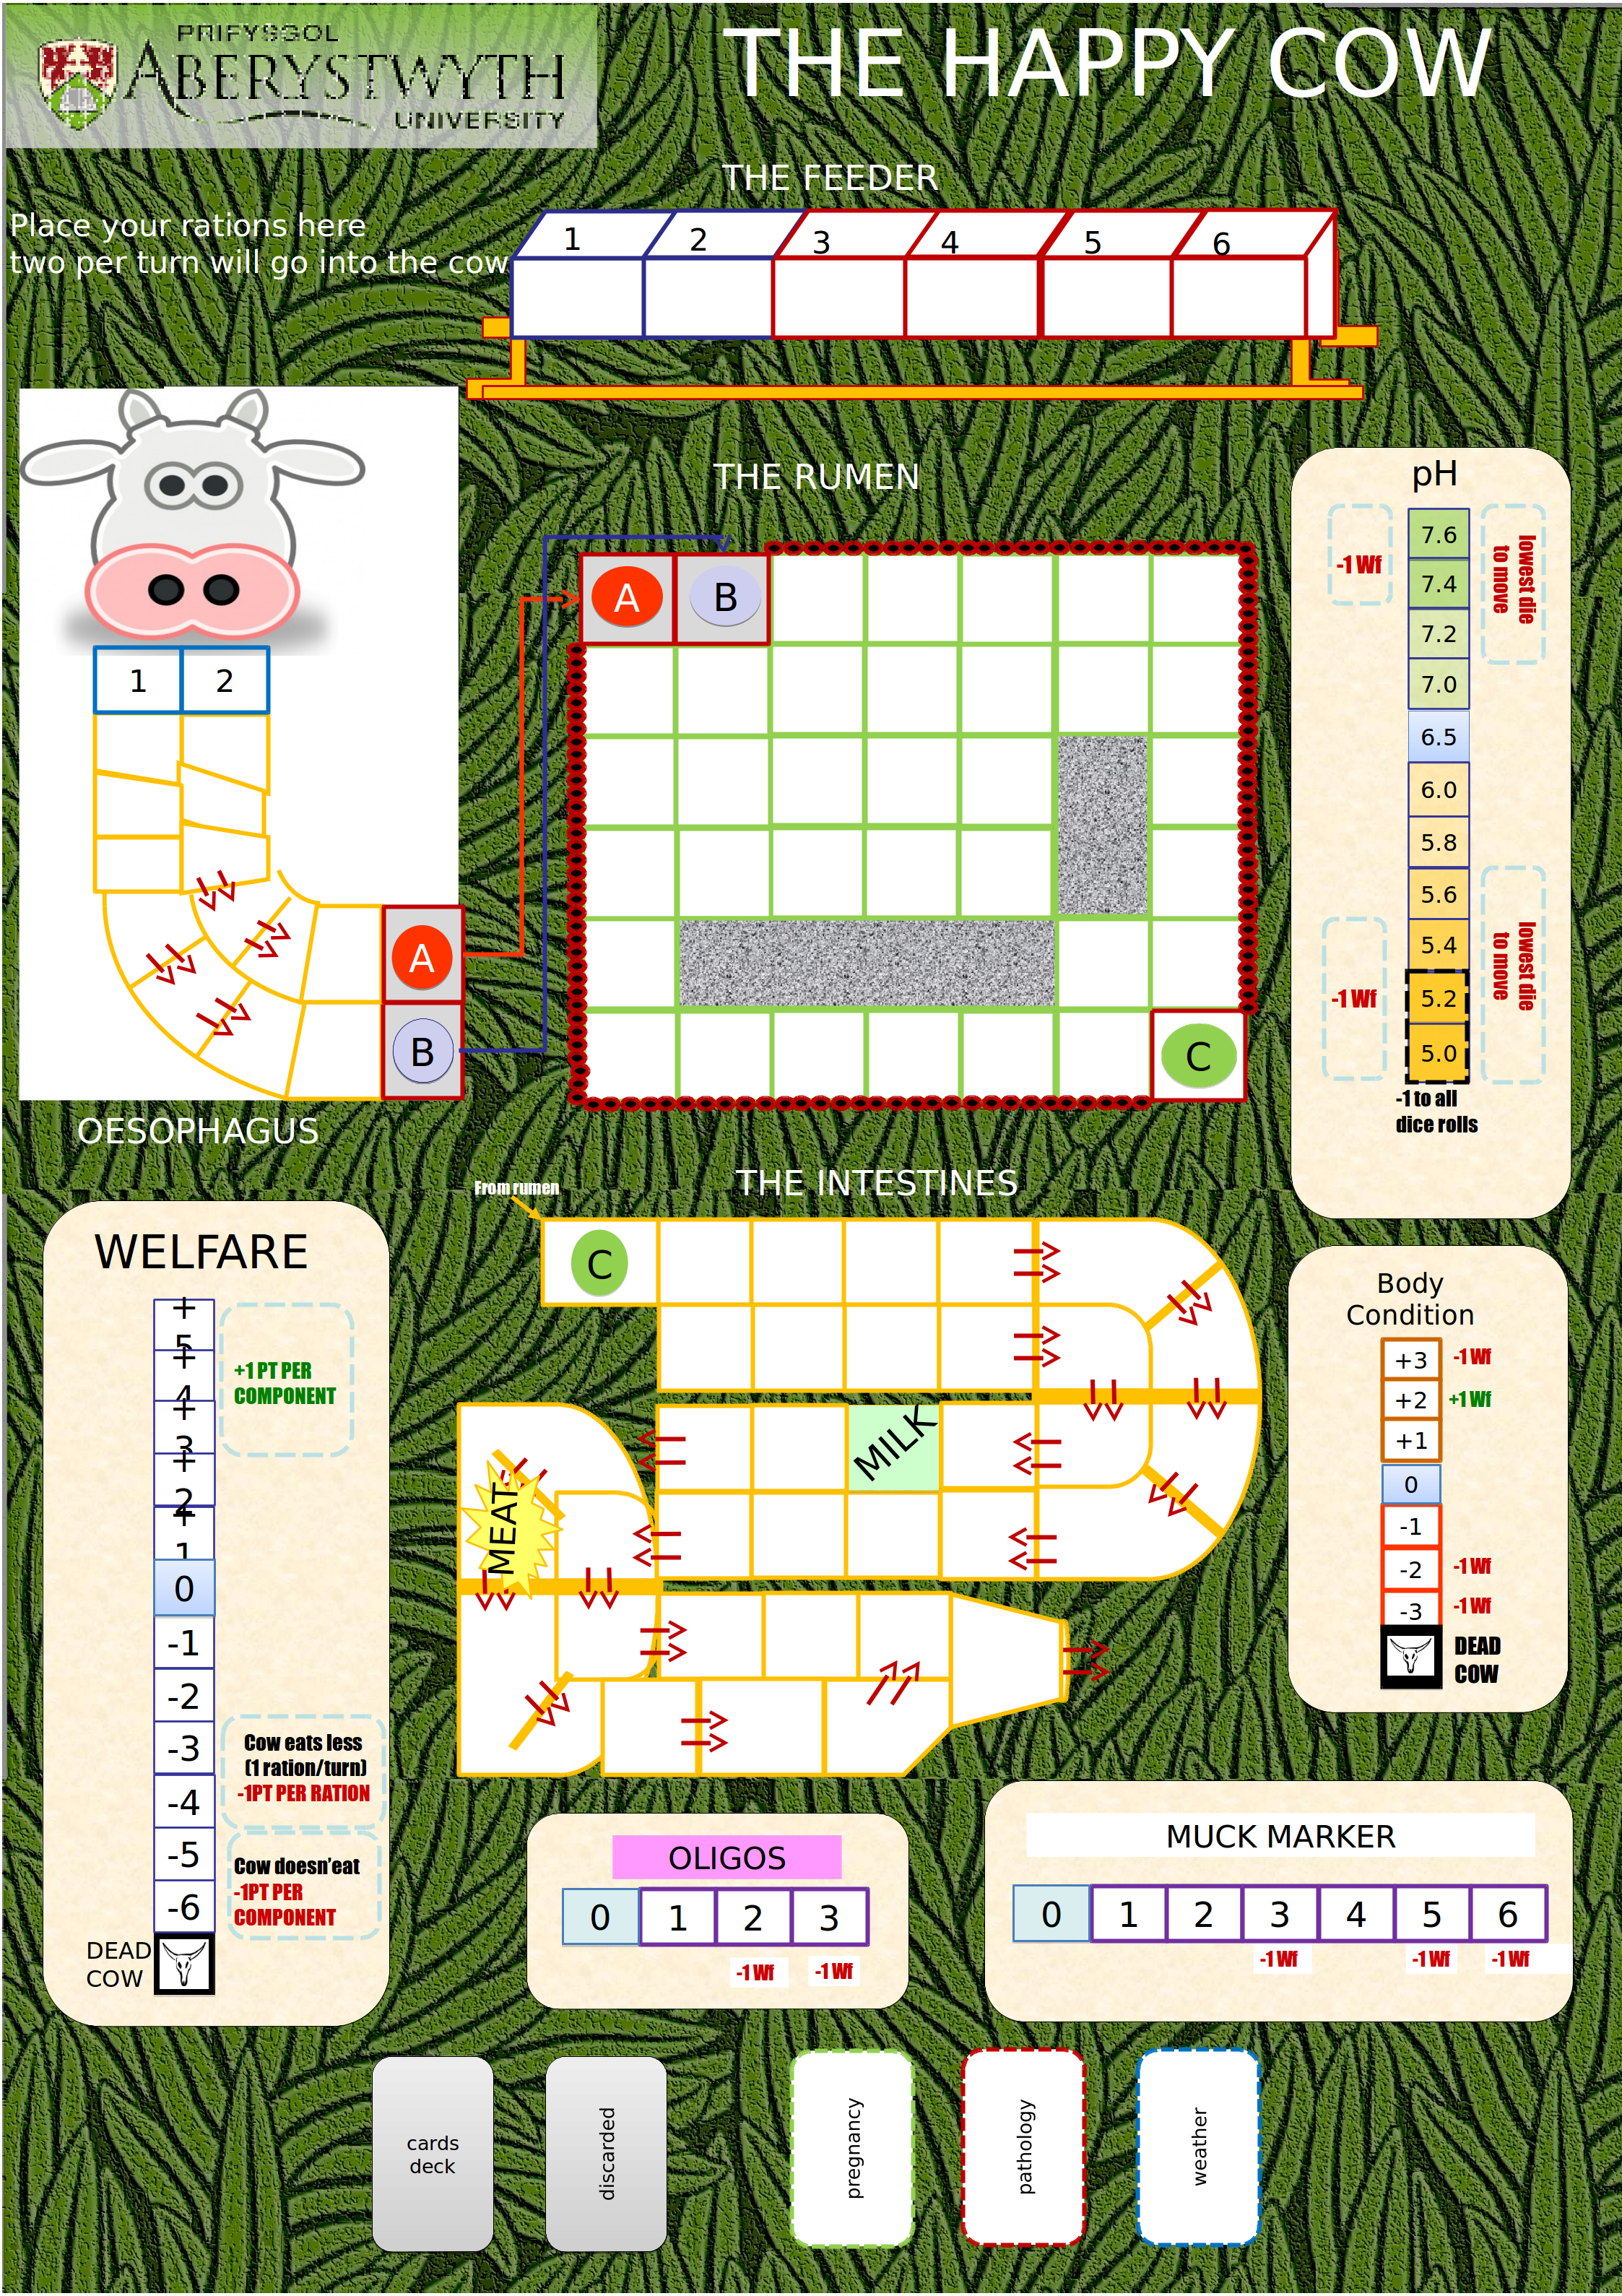
\includegraphics[width=6in]{Images/2/game-board}
\caption{The original game board. Players would sit around this and watch eachother move pieces. This is not possible with a web application where users can play accross a network.}
\label{2_play_board}
\end{figure}

When designing the user interface for the game play area, the aim was to keep these features, while also adding information about the current stage of the game (what round and turn it is), and a game menu. These details needed to be included, as they are remembered by players of a board game, but are more difficult to remember when playing a game online.

To organise the information that a user has to view and understand, three sections were created: a game information section, the current phase section, and a cow information section. These were laid out as shown in figure \ref{2_play_sections}. The purpose of each of these three sections is different, and so aims to compartmentalise the information it holds.

\begin{figure}[ht]
\centering
\includegraphics[width=6in]{Images/2/ui-sections}
\caption{This shows an early design of the user interface. There are three main sections: game information, cow information, and the current phase.}
\label{2_play_sections}
\end{figure}

Game Information provides information about the control and stage of the game. It is a menu bar, with buttons giving access to more options, such as details about player's scores and a history of the game. It gives a snapshot of the current stage of the game by stating what the round number is, by giving access to view the different phases within the round, and by showing the current active player (who's turn it is).

The Cow Information section keeps the crucial information about the cow in a static place. In the board game this information was on the board, where it can be easily seen by all. However, screens present a different scenario, one example is that they are limited in size. Fixing this information by the digestive system on a screen would make it much harder to find, and would probably involve scrolling back and forth. Instead it is fixed to the side of the screen, so it can be reviewed as the game progresses.

The two sections just mentioned provide information about the state of the game and cow. The Current Phase section contains the controls of the game. Players can select options, click buttons and drive the game forward by interacting with this section. There are four phases each round, so this section cycles through them in order, waiting for players to confirm choices before moving on to the next. The other two sections only react to changes that occur here.

The code that makes this all possible also needs to be organised. The Angular framework assigns controllers to the view by adding the controller name to an element of the DOM. All child elements are then within the scope of that controller. When the controller's data (model) changes, only the child elements within the controller will change. Controllers can be nested inside each other, and good practice suggests that each area of an application with a few controls has its own controller \cite{Angular}. This makes sure the code is adequately modulated.

Each of the sections identified above, therefore, was assigned a controller, and had a number of sub-controllers. Details of these are outlined in the design specification.

\section{Detailed Design Sections}
The design specification also considered two aspects of the application perceived to be complex, yet part of the core functionality: drawing and moving food rations, and ordering positions for pushing rations. Digging deeper into these two problems provided the outline of a solution, which helped plan the database structure and API of the application accordingly. By covering these sections in more detail the unknowns of the project were broken down into smaller problems, which could more easily be solved.

\subsection{Drawing and Moving Rations}
Food rations need a place on the screen, corresponding to their position in the cow's digestive system. On a physical board, rations would be moved from one square representing a position to another. On the screen however, the board is represented by a picture. In order to create the concept of a position a coordinate must be stored in the database. This was easily accomplished by creating the positions table, as described above. Each ration therefore has one and only one position, and the position defines where it should appear using x and y coordinates. See figure \ref{2_detail_coords}.

\begin{figure}[ht]
\centering
\includegraphics[width=6in]{Images/2/detail-1}
\caption{The original game board. Players would sit around this and watch eachother move pieces. This is not possible with a web application where users can play accross a network.}
\label{2_detail_coords}
\end{figure}

Using this structure food rations can be drawn on the screen, but that is only half the problem. Food rations also need to move through the digestive system. Users need to move rations from one position to another until they have used up their available moves. For this to be possible each position needs to know it's neighbour. An efficient way of accomplishing this is to use a graph data structure, as in figure .

\begin{figure}[ht]
\centering
\includegraphics[width=2in]{Images/2/detail-graph}
\caption{A graph has a number of nodes, which represent positions, and links, which join positions. An example of a graph is a road map, where nodes are towns and links are the roads between them.}
\label{2_detail_graph}
\end{figure}

A graph is a collection of objects, each with a number of links. Each link connects two objects. In this case the objects are positions, with coordinates, and the links are values in a joining table. It is important that links are one-directional, as in the oesophagus and intestines rations can only move one way. To accomplish this, each link has a 'from' value and a 'to' value. When searching for neighbours of a position, only links with the 'from' value coming from the current position are valid neighbours. For bi-directional links, two links are needed pointing opposite directions.

\begin{figure}[ht]
\centering
\includegraphics[width=5in]{Images/2/detail-links}
\caption{Two types of links are shown here. On the left is a uni-directional link, the graph cannot be traversed from position 2 to position 1. On the right is a bi-directional link, the graph can be traversed from either position to the other.}
\label{2_detail_links}
\end{figure}

To calculate the possible locations a food ration can reach in a certain number of moves, an algorithm is needed to traverse the graph. Starting with a position, the algorithm must visit all neighbouring positions and check the links of that next position. This is continued recursively until a depth of the number of moves given is reached. An example is given in figure \ref{2_detail_search}. 

\begin{figure}[ht]
\centering
\includegraphics[width=6in]{Images/2/detail-2}
\caption{The ration is on position 16 and can move two spaces. So beginning with position 16, position 17 is checked, leading to position 18, where the algorithm finishes. If either of these positions had more than one link, the linked positions would also be added to the result.}
\label{2_detail_search}
\end{figure}

\subsection{Ordering Positions}
The second problem concerns the order of positions, there are a two reasons for positions to have an order. Some positions have a special significance. The trough is one example, as rations in the trough are automatically moved to the front until they enter the cow. Another example is the meat and milk positions. If a ration ends its moves on one of these two positions, it is absorbed, removed, and the owner is given points. Positions therefore need a number that is not the id, so that a few of them can be recognised by the system.

The second reason is for ordering rations as they are displayed to the player. It would be possible to use the graph to calculate the order of positions, however, this is computationally expensive. If each position has a number, which increases the further down the digestive system the ration is, this provides a way to order rations based on their position.

\begin{figure}[ht]
\centering
\includegraphics[width=6in]{Images/2/detail-3}
\caption{A proposed ordering of the positions within the rumen, in the inital design specification. This changed slightly during implementation.}
\label{2_detail_order}
\end{figure}

A further use of ordering positions was outlined in the design specification: calculating where a ration should land if it gets pushed from its position. The aim was to use the order to work out directions based on the difference between the order value of neighbouring positions. However, this was proven to be inaccurate and unnecessary. Positions already have reference to their location using x and y coordinates, therefore directions can be calculated with these values.

Both these problems proved more complicated than expected, therefore changing design as they were implemented. That will be explained in the following chapter, concerning the realisation of the design in the implementation of the project.